\documentclass[12pt]{extarticle}
\usepackage[utf8]{inputenc}
\usepackage{ebgaramond}
\usepackage[export]{adjustbox}
\usepackage{eso-pic, graphicx}
\usepackage[margin=0.5in]{geometry}
\geometry{
  paperheight=210mm,
  paperwidth=147mm,
  heightrounded,
}
\usepackage{setspace}

\usepackage{pgfornament}

\usepackage{subcaption}
\usepackage{transparent}
\usepackage{verse}

\newcommand{\attrib}[1]{%
\nopagebreak{\raggedleft\footnotesize #1\par}}
\renewcommand{\poemtitlefont}{\normalfont\large\itshape\centering}

\pagenumbering{gobble}
\setlength\parindent{0pt}

\newcommand\AtPageUpperRight[1]{\AtPageUpperLeft{%
 \put(\LenToUnit{\paperwidth},\LenToUnit{0\paperheight}){#1}%
 }}%
\newcommand\AtPageLowerRight[1]{\AtPageLowerLeft{%
 \put(\LenToUnit{\paperwidth},\LenToUnit{0\paperheight}){#1}%
 }}%

\usetikzlibrary{chains, scopes}

\begin{document}


    \newcommand{\lleaf}{
        \node [on chain, xshift=-0.22cm, yshift=-0.2cm] {
            
\begin{tikzpicture}
                \node [rotate=-15] {\pgfornament[width=0.5cm]{1}};
            \end{tikzpicture}
        };
    }

    \newcommand{\linvleaf}{
        \node [on chain, xshift=-0.22cm, yshift=0.2cm] {
            
\begin{tikzpicture}
                \node [rotate=195] {\pgfornament[width=0.5cm, symmetry=v]{1}};
            \end{tikzpicture}
        };
    }

    \newcommand{\leaf}{
        \node [on chain, xshift=-0.22cm, yshift=0.2cm] {
            
\begin{tikzpicture}
                \node [rotate=-195] {\pgfornament[width=0.5cm]{1}};
            \end{tikzpicture}
        };
    }

    \newcommand{\invleaf}{
        \node [on chain, xshift=-0.22cm, yshift=-0.2cm] {
            
\begin{tikzpicture}
                \node [rotate=15] {\pgfornament[width=0.5cm, symmetry=v]{1}};
            \end{tikzpicture}
        };
    }

\newcommand{\leafline}{
\tikzset{pgfornamentstyle/.style={%
draw=black!90,inner sep=0pt,fill=black!90,
fill opacity=1,scale=1,thin}}
    \begin{tikzpicture}
    \node[inner sep=0] (A) at (0,0){};
    \coordinate (B) at (8,0);
    {
        [start chain,node distance=0,inner sep=0]
        \lleaf
        \linvleaf
        \lleaf
        \linvleaf
        \lleaf
        \linvleaf
        \lleaf
        \linvleaf
        \lleaf
        \linvleaf
        \lleaf
        \linvleaf
    }
    \end{tikzpicture}
    \begin{tikzpicture}
     \node [inner sep=0pt] at (0,0) {
\includegraphics[width=0.8cm]{mother_black.png}};
    \end{tikzpicture}
    \begin{tikzpicture}
    \node[inner sep=0] (A) at (0,0){};
    \coordinate (B) at (8,0);
    {
        [start chain,node distance=0,inner sep=0]
        \leaf
        \invleaf
        \leaf
        \invleaf
        \leaf
        \invleaf
        \leaf
        \invleaf
        \leaf
        \invleaf
        \leaf
        \invleaf
    }
    \end{tikzpicture}
}


\topskip0pt
\vspace*{\fill}

\begin{figure}[h!]
\centering
\frame{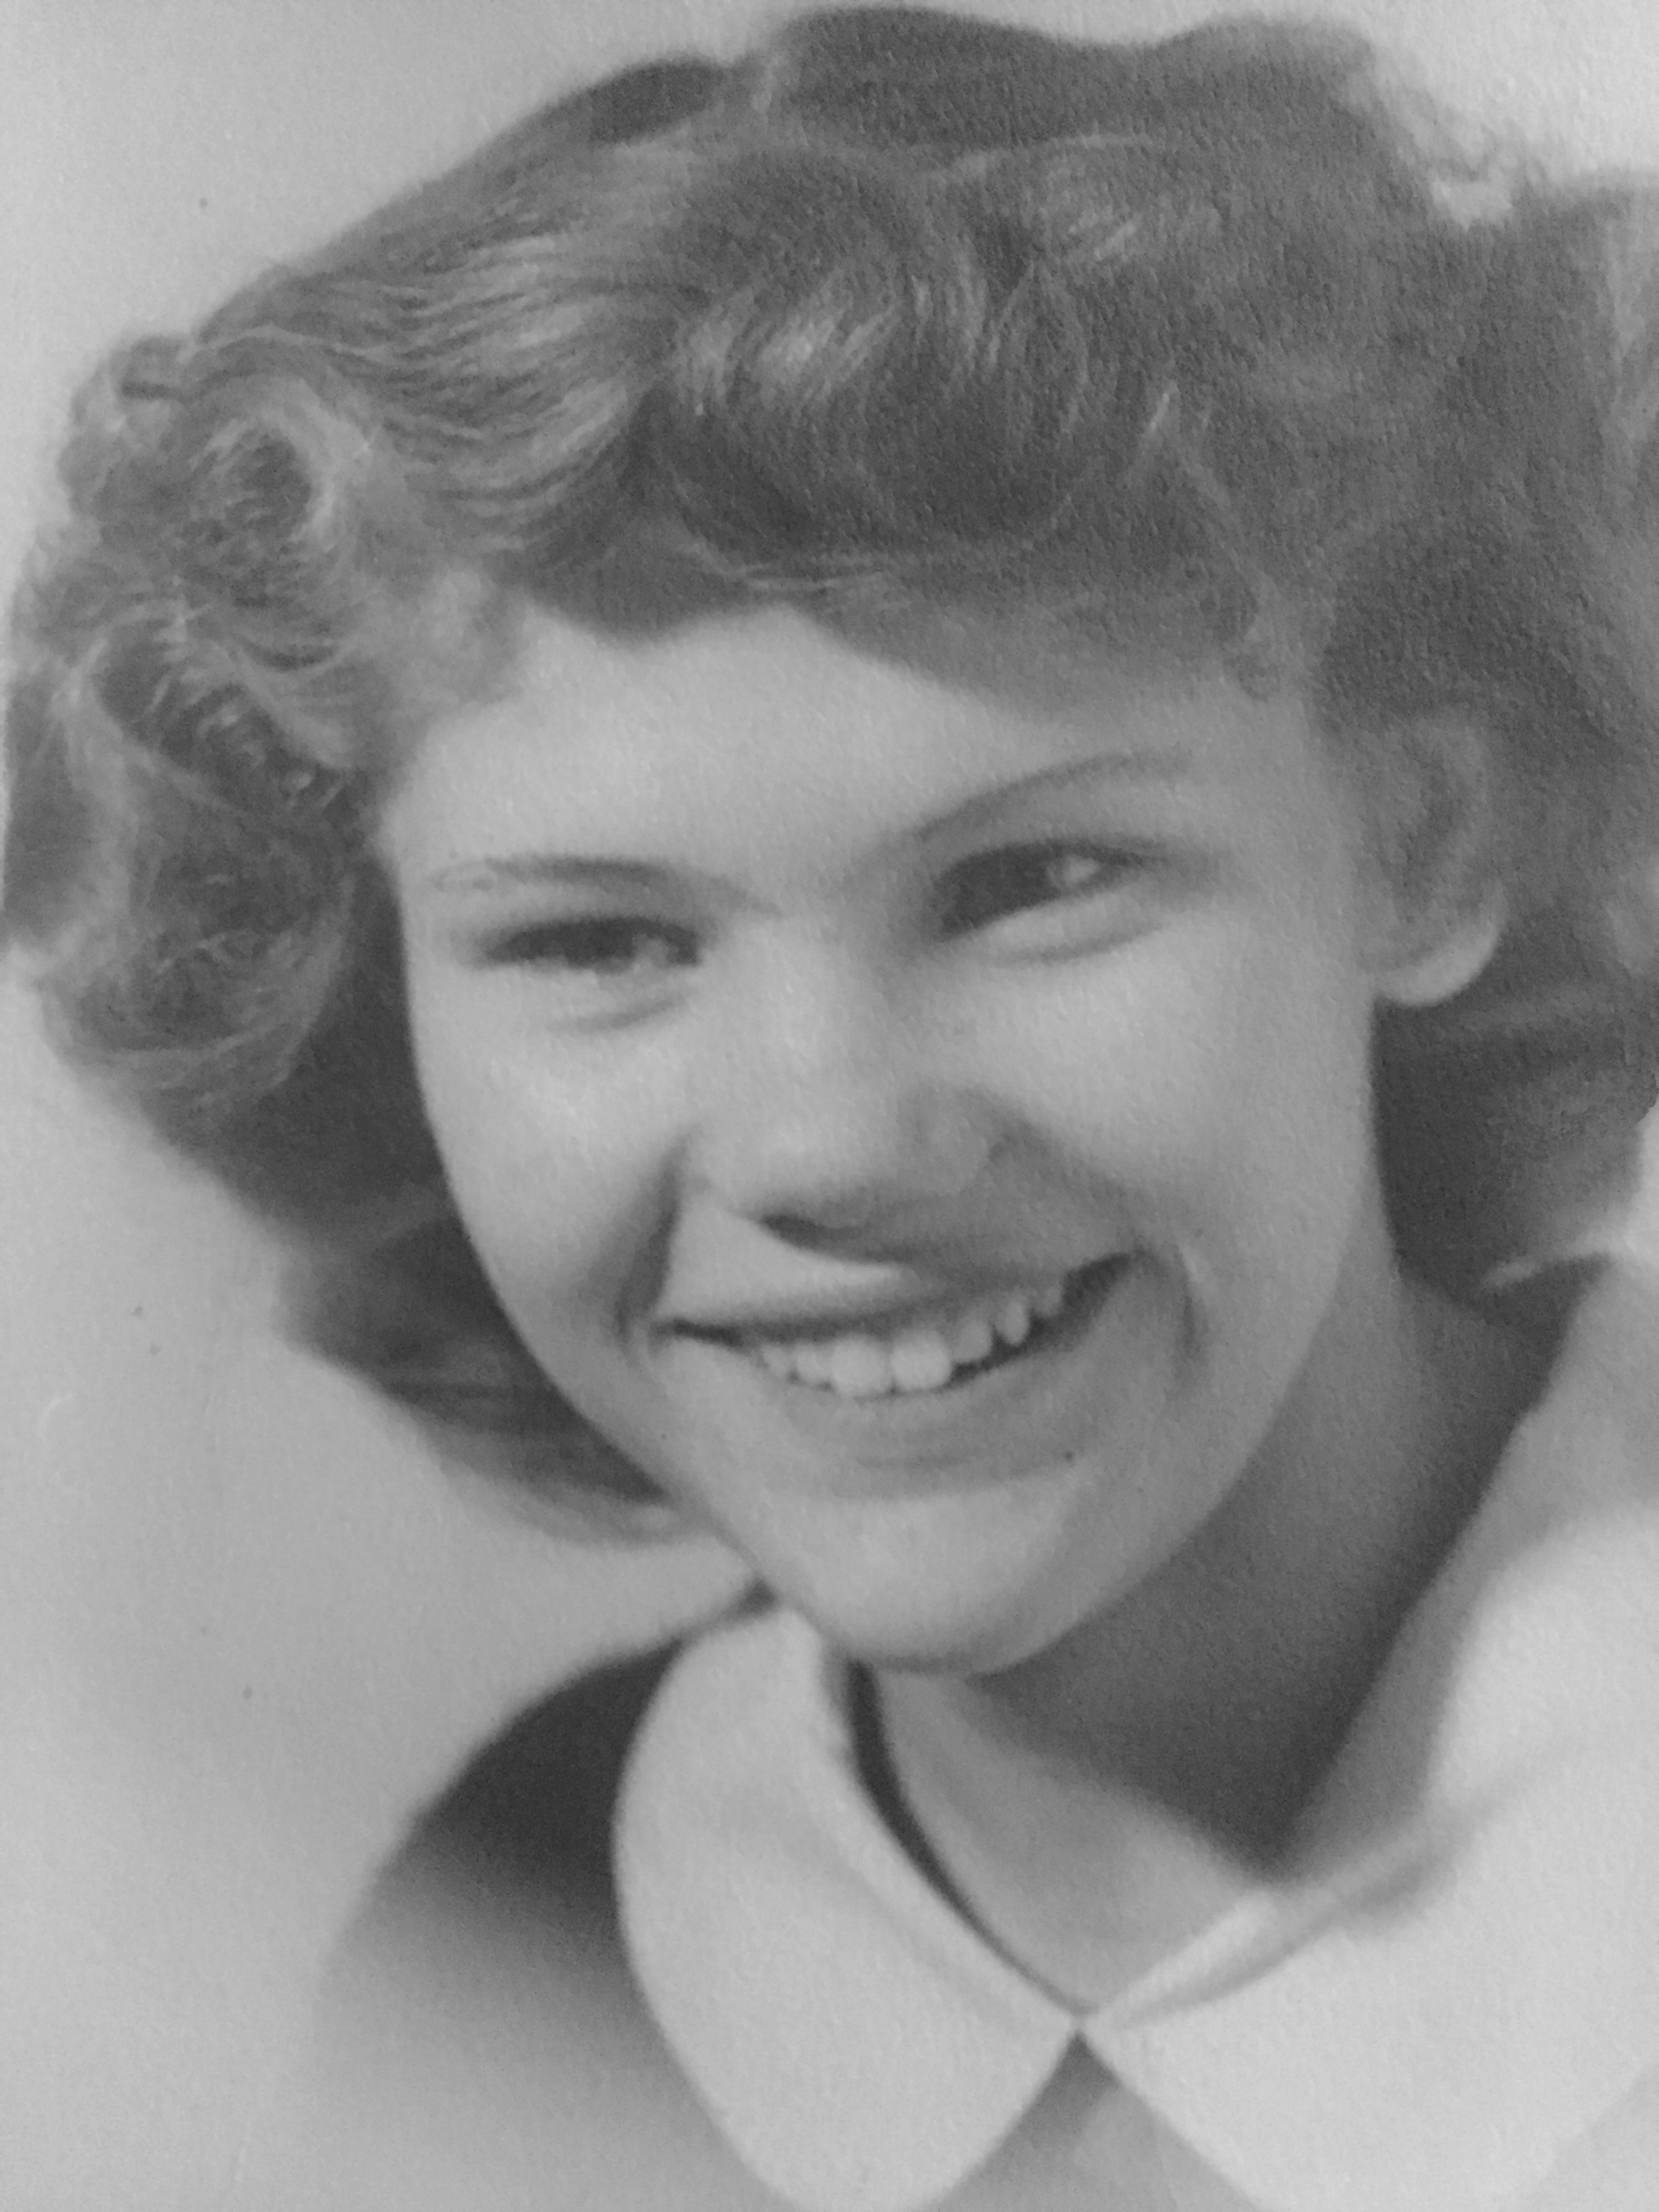
\includegraphics[width=8cm]{pg1.png}}
\end{figure}

\begin{center}
\leafline
\end{center}

{\centering \huge First name Last name \par}
{\centering \Large December 00, 0000 -- May 00, 0000 \par}

\vspace*{\fill}

% Base ornaments in corners
%\AddToShipoutPictureBG*{%
%   \AtPageUpperLeft{\put(0,-21){\pgfornament[width=1.5cm]{61}}}
%   \AtPageUpperRight{\put(-42,-21){\pgfornament[width=1.5cm,symmetry=v]{61}}}
%   \AtPageLowerLeft{\put(0,21){\pgfornament[width=1.5cm,symmetry=h]{61}}}
%   \AtPageLowerRight{\put(-42,21){\pgfornament[width=1.5cm,symmetry=c]{61}}}
%}

% \AddToShipoutPictureBG*{%
%    \AtPageUpperLeft{\put(30,-51){\pgfornament[width=1.5cm]{61}}}
%    \AtPageUpperRight{\put(-72,-51){\pgfornament[width=1.5cm,symmetry=v]{61}}}
%    \AtPageLowerLeft{\put(30,51){\pgfornament[width=1.5cm,symmetry=h]{61}}}
%    \AtPageLowerRight{\put(-72,51){\pgfornament[width=1.5cm,symmetry=c]{61}}}
% }

\newpage
\topskip0pt
\vspace*{\fill}

\begin{figure}[h!]
\centering
\frame{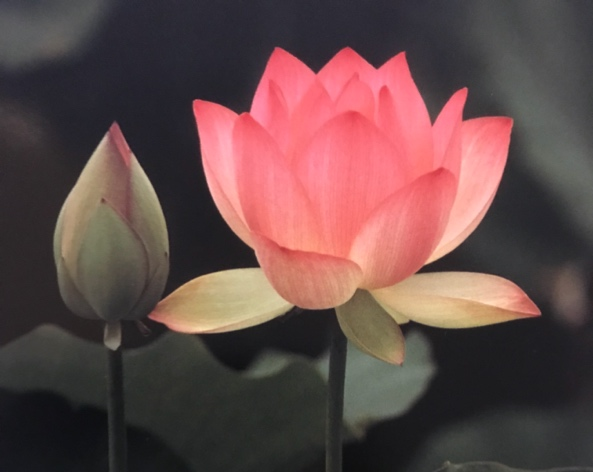
\includegraphics[width=5cm]{pg2.png}}
\end{figure}

\settowidth{\versewidth}{Who had found their common and mysterious home.}
\begin{verse}[\versewidth]
{\setstretch{1.4}\itshape
In the orchestral largeness of his mind \\
All contrary seekings their close kinship knew, \\
Rich-hearted, wonderful to each other met, \\
In the mutual marvelling of their myriad notes \\
And dwelt like brothers of one family \\
Who had found their common and mysterious home. \\
As from the harp of some ecstatic god, \\
There springs a harmony of lyric bliss \\
Striving to leave no earthly joy unsung, \\
Such was the life in that unbodied light. \\
He seemed the wideness of a boundless sky, \\
He seemed the passion of a sorrowless earth, \\
He seemed the burning of a world-wide sun. \\
}
\end{verse}
\attrib{Sri Aurobindo --- \emph{Savitri}}


\AddToShipoutPictureBG*{%
   \AtPageUpperLeft{\put(18,-72){\pgfornament[width=1.5cm]{141}}}
   \AtPageUpperRight{\put(-61,-72){\pgfornament[width=1.5cm,symmetry=v]{141}}}
   \AtPageLowerLeft{\put(18,60){\pgfornament[width=1.5cm,symmetry=h]{141}}}
   \AtPageLowerRight{\put(-61,60){\pgfornament[width=1.5cm,symmetry=c]{141}}}
}

\vspace*{\fill}

\newpage
\topskip0pt

\vspace*{\fill}

\begin{center}
\leafline


{\setstretch{1.5}
\vspace{1.5cm}
{\huge Welcome}

Mere Man Ke Andh Tamas Mein

\vspace{1.5cm}
{\huge Tributes}

First Last name

First Last name

First Last name

First Last name

First Last name


\vspace{1.5cm}
{\huge Reflection}

Guru Maat Pita Guru Bandhu Sakha

Aum Namo Bhagavate Sri Aravindaya

}
\end{center}


% \vspace*{\fill}

\AddToShipoutPictureBG*{%
	\AtTextLowerLeft{%
		\raisebox{.5\textheight}{%
			\hspace*{.5\textwidth}%
			\makebox[0pt]{{\transparent{0.35}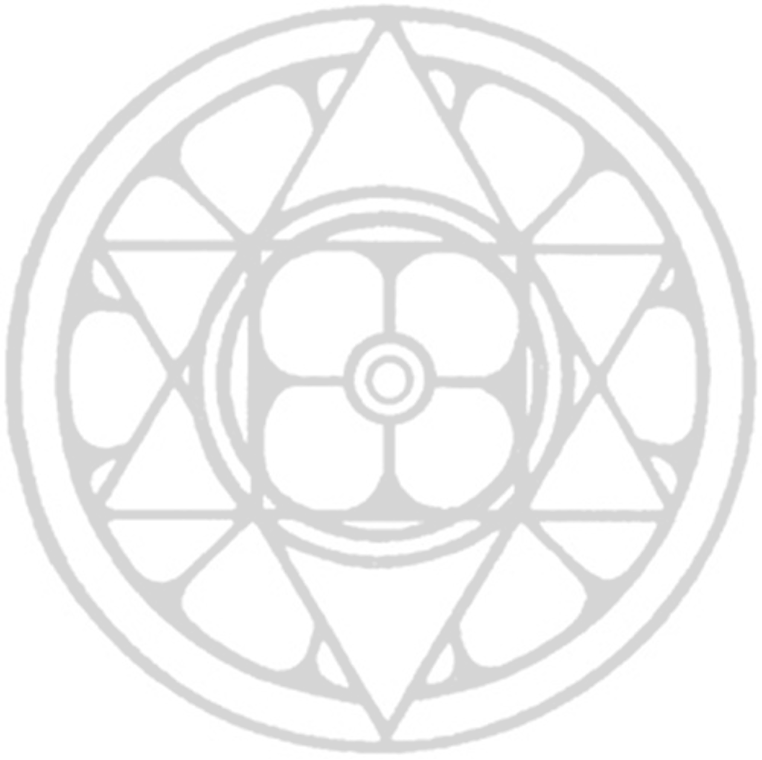
\includegraphics[width=1.1\textwidth, valign=c]{watermark.png}}}%
		}%
	}%
}


\vspace{1.5cm}

\begin{center}
\leafline
\end{center}

% \vspace*{\fill}

% \clearpage
\newpage
\topskip0pt
\vspace*{\fill}

\begin{figure}[h!]
\centering

\includegraphics[width=3.5cm]{aurobindo.png}
\end{figure}

\vspace*{\fill}

\begin{figure}[h!]
\centering
\frame{
\includegraphics[width=10cm]{pg4.jpg}}
\end{figure}

\begin{center}
\huge{Be well, be happy.}
\end{center}

\vspace*{\fill}

\begin{figure}[h!]
\centering

\includegraphics[width=3cm]{mother.png}
\end{figure}


% \AddToShipoutPictureBG*{%
%    \AtPageUpperLeft{\put(30,-51){\pgfornament[width=1.5cm]{61}}}
%    \AtPageUpperRight{\put(-72,-51){\pgfornament[width=1.5cm,symmetry=v]{61}}}
%    \AtPageLowerLeft{\put(30,51){\pgfornament[width=1.5cm,symmetry=h]{61}}}
%    \AtPageLowerRight{\put(-72,51){\pgfornament[width=1.5cm,symmetry=c]{61}}}
% }

\vspace*{\fill}
\end{document}
